\chapter{PS board品質保証試験に向けたコンパクトDAQシステムの開発}
\label{chap_QAQC}

\section{PS board QAQC試験設計}
\label{sec_QAQCdesign}
\subsection{Phase2 upgradeに向けたPS board量産スケジュール}
\ref{chap_TGC}章で述べたように、2029年から始まる高輝度LHC-ATLAS実験に向けてTGC検出器エレクトロニクスは刷新される。
TGC検出器フロントエンドエレクトロニクスの一つであるPS boardは、Run3までに使用されていたエレクトロニクスと取って代わり、FPGAを搭載した新しいハードウェアデバイスへと置き換えられる。
図\ref{PSBschedule}にPS boardの量産スケジュールを示す。PS boardは第一試作機、第二試作機の開発・調査の末、2022年にプレ量産が完了している。2024年から1400枚に及ぶ本量産が開始され、2026年からUX15へのインストール作業が行われる。
\ref{chap_TGC}章に述べたようにPS boardはTGC検出器上に直接取り付けられたPSパックと呼ばれる領域に設置される。そのため一度加速器での陽子衝突が始まると修理や交換が極めて困難となる。TGC検出器を安定的に動作させ、検出器としての不感領域を最小限に抑えるためには、量産された各個体それぞれにハードウェアの初期不良がないことを詳細に調べ上げた上でインストールすることが大切となる。そのために行う一連の品質調査試験のことを一般にQuality Assurance and Quality Control (QAQC)試験と呼ぶ。本章ではPS board QAQC試験の設計やそれに際して開発したコンパクトDAQシステムの概要・実装・検証について述べる。

\begin{figure} 
\centering
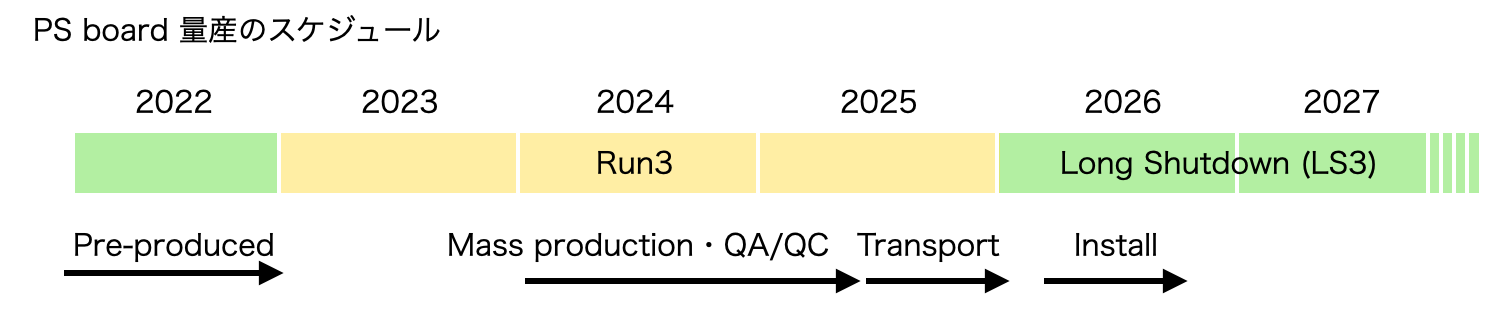
\includegraphics[width=14cm]{fig/PSBschedule.png}
\caption[PS board量産のスケジュール]{PS board量産のスケジュール。PS boardはこれまでに第一試作機、第二試作機を通したシステム開発が完了いる。2023年現在、プレ量産された各個体に対しての試験を進めている。2024年から1400枚の本量産が開始され2026年から実験室への設置が開始される。}
\label{PSBschedule}
\end{figure}

\subsection{PS board QAQC試験の設計}
\label{subsec_QAQCdesign}
QAQC試験ではエレクトロニクス上のすべての素子を網羅的に検証することが必要となる。
以下にPS boardに搭載されている各素子と各素子間の配線を示す。

\begin{figure} 
\centering
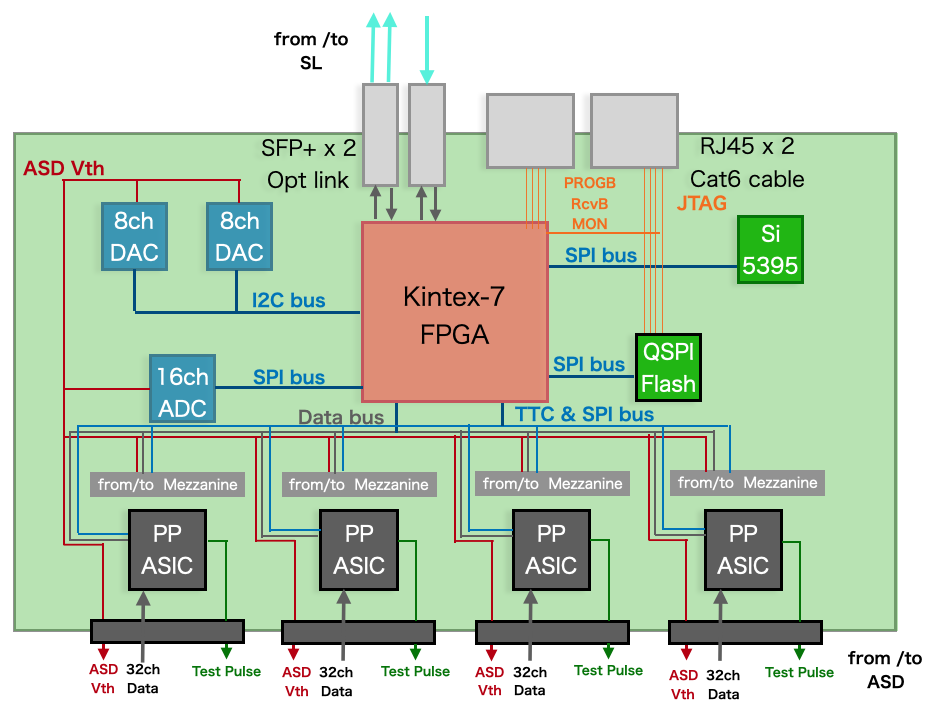
\includegraphics[width=14cm]{fig/PSBoverall.png}
\caption[PSboardの全体像]{PS boardの全体像。PS boardに搭載されている各素子とその間の配線を示している。PS boardはSLと光ケーブル、JATHubとCat6ケーブルで接続される。PS board FPGAとDAC、ADC、Si5395、QSPI、PPASICはI2CまたはSPIバスで接続される。DACからアナログ信号として供給される閾値電圧は8台のASDボードとモニター用のADCに分配される。FPGAはPPASICにTTC信号を送信し、ヒット信号を受信する。1つのPPASICは2台のASDボードと接続されテストパルス信号を送信し、それぞれから8チャンネル分のヒットデータを受信する。}
\label{PSBconcept}
\end{figure}

\vskip0.5\baselineskip

\textbf{PS board FPGAとの配線}
\begin{enumerate}
    \item \texttt{光ケーブル経由でのSLとの通信 :} PS boardからの送信用として2リンク、SLからの受信用として1リンクが用意されている。SLから16 Gbpsで送られる光信号はSFP+モジュール内で電気信号へと変換され、FPGAに搭載されている高速シリアル通信対応のトランシーバーの一種である7シリーズGTXトランシーバーで受信される。SLからPS boardへはコントロール信号が配られ、これに乗せてTTC信号も分配される。PS boardからSLへは256チャンネル分のヒット信号が40 MHzおきに送信される。
    \vskip0.5\baselineskip

    \item \texttt{Cat6ケーブル経由でのJATHubとの通信 :} PS boardは2本のCat6ケーブルでJATHubと接続される。一本はJTAGパスと呼ばれJATHubからJTAGプロトコルでPS board FPGAやQSPIフラッシュメモリーへファームウェアを書き込む際に使用される。もう一本はRecoveryパスと呼ばれる。RecoveryパスはPROGB線、RcvB線、MON線、GTX reset線、の4本のLVDS信号で構成される。PS board FPGA内で修復可能なSingle Event Upset(SEM)が生じた場合、PS boardはRcvB線を通じて救難信号を送信し、JATHubからファームウェアリセットのための信号をPROGB線を通じて受信する。また、PS boardで再構成したLHCバンチ交差クロックをMON線を通じてJATHubへ送信し、JATHubに接続される11台のPS board間の相対的な位相関係を測定する。
    \vskip0.5\baselineskip

    \item  \texttt{I2Cバス経由でのDACとの通信 :} PS board FPGA は I2C プロトコルを介して DAC の制御を行う。ASDにかけられる閾値電圧の極性や絶対値はこのパスを通じて制御される。
    \vskip0.5\baselineskip

    \item \texttt{SPIバス経由でのQSPI フラッシュメモリーとの通信 :} PS board FPGAはSPIプロトコルを介してQSPI フラッシュメモリーへの読み書きを行う。PPASIC制御用レジスタに格納される値、DACの閾値電圧や極性などのパラメーターはこのメモリーに格納されており、電源投入時にこれらのパラメーターは各素子へと分配されるよう設計されている(自立型制御機構)。
    \vskip0.5\baselineskip
    
    \item \texttt{SPIバス経由でのSi5395との通信 :} PS board FPGA はSPIプロトコルを介してSi5395の制御を行う。自立型制御機構のシークエンスの中でFPGA内部に格納された制御用パラメーターがこのパスを通じてSi5395に送られ、クロックの入出力や周波数の設定が行われる。またFPGA内部で再構成されたLHCバンチ交差クロックはSi5395に入れられジッターの低減が行われた後にFPGAやGTXトランシーバーへと分配される。
    \vskip0.5\baselineskip

    \item \texttt{SPIバス経由でのADCとの通信 :} PS board FPGAはSPIプロトコルを介してADCからのデータ読み出しを行う。ADCはDACからASDに印加される閾値電圧をモニターしており、ADCによって読み出された電圧値はこのパスを通じてFPGAへと伝達される。
    \vskip0.5\baselineskip

    \item\texttt{PPASICとの通信 :} PS board FPGAはSPIプロトコルを介してPPASICの制御を行う。~\ref{chap_TGC}~章で述べたようにPPASICはASDから送られるヒット信号のデジタル化を担当しており、ヒット信号に対するディレイの大きさやBCIDゲートの幅などのパラメーターはこのパスを通じてFPGAから行われる。その他にもFPGAからPPASICへのTTC信号やテストパルストリガー信号、PPASICからFPGAへのヒット信号の送信のためのパスも用意されている。
    \vskip0.5\baselineskip
\end{enumerate}

\textbf{その他の素子間での配線}
\begin{enumerate}[resume]
    \item \texttt{DACからASD、ADCへの閾値電圧の分配} 
    \vskip0.5\baselineskip

    \item \texttt{PPASICとASDの通信 :} 1つのPPASICは2台のASDボードと接続されテストパルス信号を送信し、それぞれから8チャンネル分のヒットデータを受信する。
    \vskip0.5\baselineskip
\end{enumerate}


以上の配線を網羅的に試験できる必要十分な試験として以下の項目が挙げられる。この際PS board FGPA内で使用するファームウェアは試験用のファームウェアを別に用意するのではなく、実際の運用時に使用するものと同じものを使用する。

\subsubsection{QSPIフラッシュメモリーへのファームウェア書き込み試験}
\label{subsubsec_QSPI}

\subsubsection{QSPIフラッシュメモリーへの制御パラメーター書き込み試験}
\label{subsubsec_QSPIparam}

\subsubsection{Recovery path試験}
\label{subsubsec_recovery}

\subsubsection{ADC試験}
\label{subsubsec_ADC}

\subsubsection{Clock位相測定試験}
\label{subsubsec_clock}

\subsubsection{ASDテストパルス試験}
\label{subsubsec_testpulse}







